\section{Results}\label{sec:results}

\begin{figure}[t]
\centering
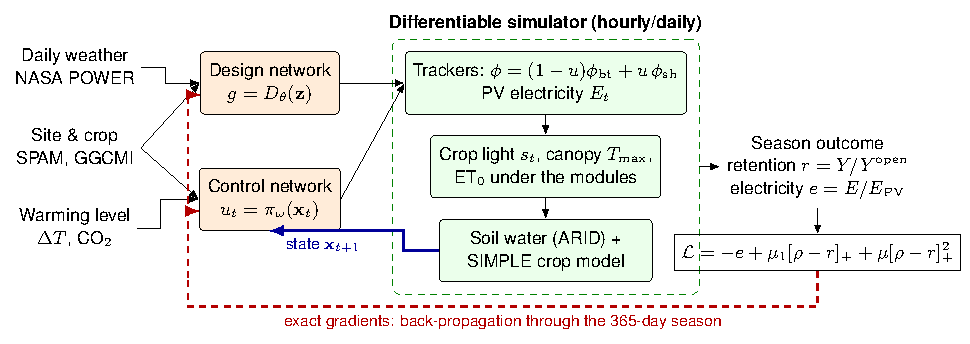
\includegraphics[width=\textwidth]{figures/scheme.pdf}
\caption{SALS. A design network chooses the ground coverage ratio $g$ of single-axis tracker rows from site descriptors, and a control network chooses the daily light-sharing level $u_t$ from the crop, soil and weather state. The differentiable simulator converts these decisions into PV electricity, light and microclimate at the crop, soil water and crop growth. The season's electricity and yield retention enter a penalised objective whose exact gradient is back-propagated through the 365-day season to both networks.}
\label{fig:scheme}
\end{figure}

\begin{figure}[t]
\centering
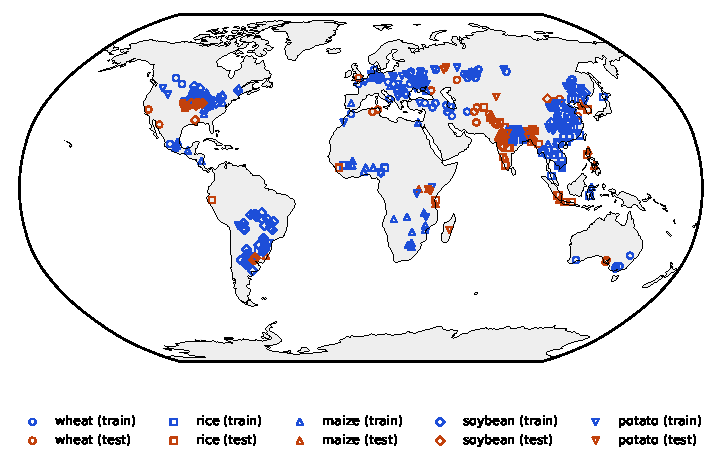
\includegraphics[width=\textwidth]{figures/sites.pdf}
\caption{The 400 crop--site pairs, sampled in proportion to the harvested area of each crop (SPAM 2010). Blue: training sites; orange: geographically held-out test sites (10\textdegree{} blocks).}
\label{fig:map}
\end{figure}

\subsection{Electricity and food on held-out sites and years}\label{sec:main}
Table~\ref{tab:main} and Fig.~\ref{fig:tradeoff} compare the methods on 461 test seasons: 2015--2019 at geographically held-out sites, excluding seasons in which the open-field crop failed ($<0.2$\,t\,ha$^{-1}$). Under the baseline climate, the static agrivoltaic designs that keep 90\% of the yield must use very sparse arrays (GCR $\approx0.10$). They produce 361--377\,MWh\,ha$^{-1}$\,yr$^{-1}$, a quarter of the electricity of a conventional PV plant, and reach an LER of 1.18--1.20. Rotating the trackers to share light with the crop allows denser arrays. The seasonal-sharing and stress rules reach 629 and 707\,MWh\,ha$^{-1}$\,yr$^{-1}$ (LER 1.37 and 1.42), even though their GCR is chosen with knowledge of the test weather. SALS chooses a GCR of 0.34 on average and produces 1019\,MWh\,ha$^{-1}$\,yr$^{-1}$, 72\% of a conventional PV plant, with a mean yield retention of 0.909. Its LER of 1.63 (95\% CI 1.57--1.70) is 0.21 higher than that of the best expert rule and 0.43 higher than that of the static design ($p<10^{-4}$, paired Wilcoxon tests, Table~\ref{tab:stats}). Per-season open-loop optimisation with perfect foresight reached an LER of 1.55. It remained below SALS because optimising 365 daily controls separately for each season is a harder, non-convex problem than learning one policy from thousands of seasons.

\begin{table}[t]
\centering
\caption{Held-out performance (test sites, seasons 2015--2019). GCR: mean ground coverage ratio; $E$: electricity (MWh\,ha$^{-1}$\,yr$^{-1}$); $e$: electricity relative to a conventional PV plant; $r$: mean yield retention; compliance: share of seasons with $r\ge0.9$; LER $=r+e$ with bootstrap 95\% CI over sites. Oracle-GCR baselines choose the GCR with knowledge of the test weather; the open-loop optimisation also knows the daily weather of each test season.}
\label{tab:main}
\small
\begin{tabular}{lcccccc}
\toprule
Method & GCR & $E$ & $e$ & $r$ & Compliance (\%) & LER [95\% CI]\\
\midrule
\multicolumn{7}{l}{\textit{Baseline}}\\
AV static (rule) & 0.10 & 361 & 0.26 & 0.920 & 60.3 & 1.18 [1.16, 1.20]\\
AV static (oracle GCR) & 0.10 & 377 & 0.27 & 0.935 & 85.2 & 1.20 [1.16, 1.25]\\
Seasonal sharing & 0.26 & 629 & 0.45 & 0.921 & 82.2 & 1.37 [1.33, 1.41]\\
Stress rule & 0.23 & 707 & 0.50 & 0.922 & 80.9 & 1.42 [1.37, 1.48]\\
SALS (ours) & 0.34 & \textbf{1019} & 0.72 & 0.909 & 49.5 & 1.63 [1.57, 1.70]\\
Open-loop (foresight) & 0.30 & 916 & 0.65 & 0.901 & 28.6 & 1.55 [1.49, 1.61]\\
\addlinespace
\multicolumn{7}{l}{\textit{+1.5\,\textdegree C}}\\
AV static (rule) & 0.10 & 355 & 0.26 & 0.924 & 66.7 & 1.18 [1.16, 1.20]\\
AV static (oracle GCR) & 0.11 & 385 & 0.28 & 0.931 & 83.5 & 1.21 [1.17, 1.25]\\
Seasonal sharing & 0.28 & 647 & 0.47 & 0.918 & 79.2 & 1.38 [1.34, 1.43]\\
Stress rule & 0.23 & 722 & 0.52 & 0.919 & 77.7 & 1.44 [1.39, 1.49]\\
SALS (ours) & 0.36 & \textbf{1079} & 0.77 & 0.901 & 46.8 & 1.67 [1.61, 1.74]\\
\addlinespace
\multicolumn{7}{l}{\textit{+2\,\textdegree C}}\\
AV static (rule) & 0.10 & 354 & 0.26 & 0.926 & 69.1 & 1.18 [1.16, 1.20]\\
AV static (oracle GCR) & 0.11 & 393 & 0.29 & 0.929 & 83.5 & 1.22 [1.17, 1.26]\\
Seasonal sharing & 0.28 & 659 & 0.48 & 0.917 & 78.9 & 1.39 [1.35, 1.44]\\
Stress rule & 0.23 & 728 & 0.53 & 0.918 & 77.2 & 1.44 [1.39, 1.50]\\
SALS (ours) & 0.37 & \textbf{1106} & 0.79 & 0.898 & 46.3 & 1.69 [1.62, 1.76]\\
\addlinespace
\multicolumn{7}{l}{\textit{+3\,\textdegree C}}\\
AV static (rule) & 0.10 & 353 & 0.26 & 0.933 & 74.2 & 1.19 [1.17, 1.21]\\
AV static (oracle GCR) & 0.12 & 442 & 0.32 & 0.927 & 80.1 & 1.25 [1.20, 1.30]\\
Seasonal sharing & 0.30 & 694 & 0.50 & 0.920 & 78.1 & 1.42 [1.38, 1.47]\\
Stress rule & 0.24 & 762 & 0.55 & 0.919 & 77.7 & 1.47 [1.42, 1.53]\\
SALS (ours) & 0.39 & \textbf{1173} & 0.85 & 0.901 & 45.1 & 1.75 [1.68, 1.82]\\
Open-loop (foresight) & 0.34 & 1028 & 0.74 & 0.901 & 25.8 & 1.65 [1.58, 1.71]\\
\bottomrule
\end{tabular}
\end{table}

\begin{figure}[t]
\centering
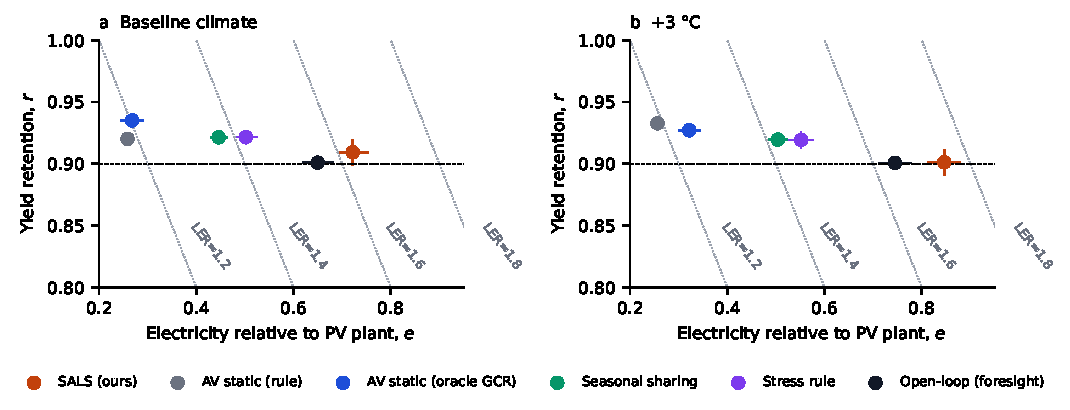
\includegraphics[width=\textwidth]{figures/tradeoff.pdf}
\caption{Electricity--food trade-off on held-out sites and years. Points are means with 95\% confidence intervals; dotted lines are iso-LER lines; the dashed line is the 90\% yield-retention floor.}
\label{fig:tradeoff}
\end{figure}

The gain comes with a trade-off that must be stated clearly. SALS meets the floor \emph{on average}: its mean retention is 0.90--0.91 in all four climates. It meets the floor in only 45--49\% of individual seasons, however, whereas the rule-based baselines meet it in 78--85\% of seasons. The penalty objective (Eq.~\ref{eq:loss}) lets SALS go slightly below the floor in some seasons in exchange for much more electricity. The rules stay above the floor with a margin (mean $r\approx0.92$) and produce 30--65\% less electricity. The floor in Eq.~\eqref{eq:problem} is a per-season constraint; a formulation that guarantees it in a given share of seasons, i.e.\ a chance constraint, would be the natural extension for deployments where regulation is enforced every season (Section~\ref{sec:limits}).

\subsection{What the policy learned}
Fig.~\ref{fig:trajectory} shows the learned control for two of the hottest test seasons under +3\,\textdegree C. For rainfed maize in the Nile Delta, SALS keeps the trackers in energy mode during crop establishment, opens them fully ($u\approx1$) during the canopy-building phase, when intercepted light is most valuable, and returns to energy mode in the second half of the season, when maximum temperatures exceed 40\,\textdegree C and the shade protects the canopy. For irrigated wheat in north-western India, it shares light throughout the cool vegetative phase and shades the crop during the hot grain-filling period before harvest. Over all active crop days of the +3\,\textdegree C test seasons, the mean light-sharing level is 0.33 on days with heat stress and 0.46 on other days. The policy has thus learned to trade light for cooling when heat, not light, limits growth. The design network chooses denser arrays for hotter and drier sites and for maize and soybean (mean GCR 0.42 and 0.39 at present climate) than for wheat and potato (0.32). In these crops, heat and drought limit yield more than light does.

\begin{figure}[t]
\centering
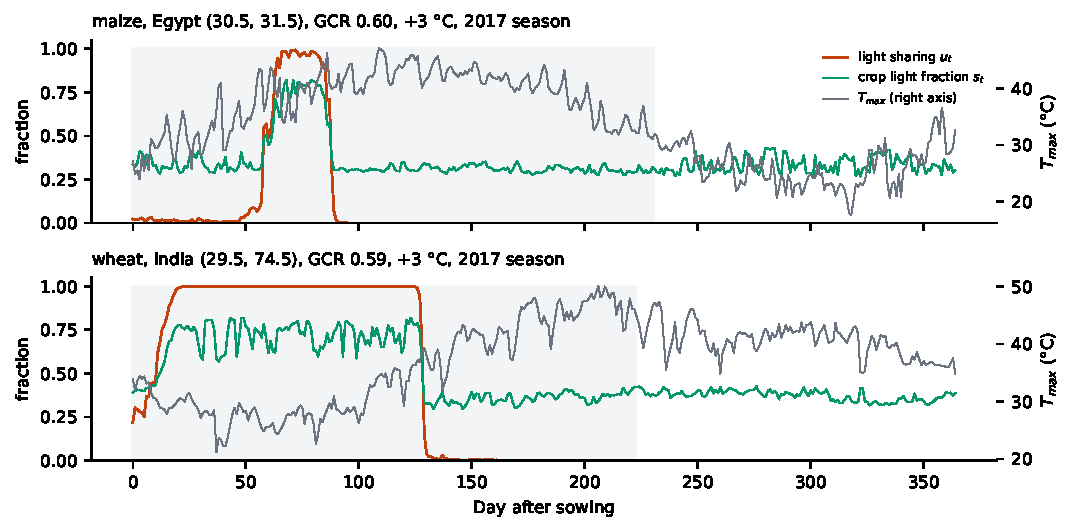
\includegraphics[width=\textwidth]{figures/trajectory.pdf}
\caption{Learned daily control for two hot test seasons under +3\,\textdegree C. Shading marks the cropping season. Orange: light-sharing level $u_t$ chosen by SALS; green: fraction of open-field irradiance reaching the crop; grey: daily maximum temperature (right axis).}
\label{fig:trajectory}
\end{figure}

\subsection{Agrivoltaics under global warming}
Warming changes the balance between light and heat. With the same trained networks, SALS increases its electricity from 1019 to 1079, 1106 and 1173\,MWh\,ha$^{-1}$\,yr$^{-1}$ at +1.5, +2 and +3\,\textdegree C (from 72\% to 85\% of a conventional PV plant) while keeping the mean retention relative to the same-climate open field at 0.90 (Table~\ref{tab:main}). Its LER rises from 1.63 to 1.75, whereas that of the static design stays at about 1.2. Two effects cause this. Warmer seasons are shorter, so the crop occupies the field for fewer days, and heat and drought stress make light less limiting, so more shade can be tolerated or is even beneficial. Across all 400 sites, the SALS system yields more than the open field in 13--14\% of seasons, rising to 31--35\% for maize and 25--28\% for soybean, mostly at hot, rainfed sites (Fig.~\ref{fig:global}b).

Agrivoltaics is not, however, a remedy for the aggregate warming damage. Summed over sites, open-field production of maize and rice falls by 18 and 17\% at +3\,\textdegree C in our simulations, and SALS production by 23 and 26\% relative to the baseline open field, i.e.\ 94 and 90\% of the same-climate open field (Fig.~\ref{fig:warming}). Potato and wheat, which benefit from warmer conditions at cool sites and from CO$_2$ fertilisation in the model, gain in the open field, and SALS keeps 87--89\% of this production. The benefit of SALS under warming is that it maintains the food-security floor while producing more electricity per hectare. It does not reverse the climate impact on yields.

\begin{figure}[t]
\centering
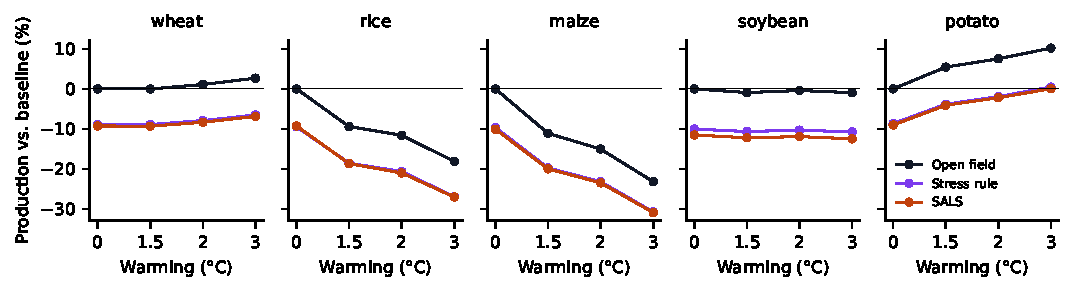
\includegraphics[width=\textwidth]{figures/warming.pdf}
\caption{Production relative to the baseline open field (sum over sites, test years) as a function of warming, for the open field, static agrivoltaics and SALS.}
\label{fig:warming}
\end{figure}

\subsection{Global electricity potential}\label{sec:global}
Fig.~\ref{fig:global} maps the electricity and LER of SALS at all 400 sites. Electricity ranges from a few hundred ha$^{-1}$\,yr$^{-1}$ at high-latitude wheat sites to more than 2000\,MWh\,ha$^{-1}$\,yr$^{-1}$ at sunny, hot maize and soybean sites in South Asia, Africa and the Americas, where the LER exceeds 2. Because the sites were sampled in proportion to harvested area, their mean electricity per hectare can be scaled to the global area of each crop. Deploying SALS agrivoltaics on 5\% of the harvested area of the five crops (33\,Mha) would generate about 31{,}000\,TWh\,yr$^{-1}$ at present climate and 37{,}000\,TWh\,yr$^{-1}$ at +3\,\textdegree C, while retaining on average 93\% of the crop yield on that land. Static agrivoltaic designs with the same yield floor would generate about 11{,}700\,TWh\,yr$^{-1}$. For comparison, global electricity generation was about 30{,}000\,TWh in 2023 \citep{ember2024}. These are technical potentials: they ignore grid integration, storage, land tenure and economic constraints (Section~\ref{sec:limits}). They show, however, that light sharing makes the food-compatible share of cropland large enough to matter for global energy security.

\begin{figure}[t]
\centering
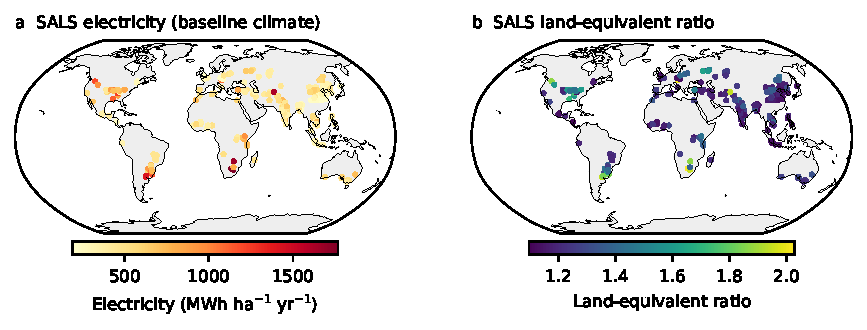
\includegraphics[width=\textwidth]{figures/map.pdf}
\caption{SALS electricity (a) and land-equivalent ratio (b) at the 400 sites (baseline climate, mean of seasons 2015--2019).}
\label{fig:global}
\end{figure}

\subsection{Sensitivity and ablation}\label{sec:sensitivity}
The canopy-cooling coefficient $\kappa$ is the most uncertain microclimate parameter. Evaluated without retraining at $\kappa=0$, 1, 2 and 3\,\textdegree C, the electricity of SALS barely changes (1026--1022\,MWh\,ha$^{-1}$\,yr$^{-1}$ at present climate). Its mean retention changes from 0.871 to 0.931 at present climate and from 0.847 to 0.927 at +3\,\textdegree C. Without any cooling benefit, the policy therefore under-shoots the floor by 3--5 points. The heat-protection effect is thus an important part of the benefit under warming, and field measurements of canopy temperature under trackers are needed to pin it down.

Table~\ref{tab:ablation} reports three ablations. Each variant was trained with the same budget of 200 steps as a reference SALS model and evaluated on the held-out seasons.

\begin{itemize}
\item \emph{Without stress features}: the control network sees only phenology, time, design and crop, with soil water, ARID and the maximum-temperature, irradiance and ET$_0$ forecasts masked. At similar mean retention, this variant produced 28\% less electricity (700 vs 971\,MWh\,ha$^{-1}$\,yr$^{-1}$) and lowered the LER from 1.59 to 1.40 at present climate and from 1.67 to 1.42 at +3\,\textdegree C. A stress-blind policy performs like the expert rules: it learns \emph{when} in the season to share light, but it cannot respond to the heat and drought of a particular season.
\item \emph{Without the design network}: every site uses a GCR of 0.3, close to the mean GCR chosen by SALS, and only the controller is learned. The LER fell to 1.42 and 1.43, and compliance dropped to 31--38\%. The benefit of SALS therefore comes from matching the array density to the site's climate and crop: denser at hot, dry sites where shade is cheap, sparser where light limits growth. The same mean density everywhere does not achieve this.
\item \emph{Trained on the baseline climate only}: the networks were trained on the present climate alone and evaluated in all four climates. They did not learn to exploit the heat-protection value of shade. Their electricity stayed at about 670\,MWh\,ha$^{-1}$\,yr$^{-1}$ and their LER at 1.38--1.40 under all warming levels, whereas the multi-climate model's LER rose from 1.59 to 1.67. This variant was weaker even under the present climate. With a single training seed we cannot separate a regularising effect of the more diverse multi-climate data from optimisation variance, but the result shows that training on projected climates is needed for a policy that remains effective as the climate warms.
\end{itemize}

Training longer (400 instead of 200 steps) added a further 0.04--0.08 to the LER.

\begin{table}[t]
\centering
\caption{Ablation on held-out seasons. $E$: electricity (MWh\,ha$^{-1}$\,yr$^{-1}$); $r$: mean yield retention; C: compliance (\% of seasons with $r\ge0.9$). All ablations were trained for 200 steps and should be compared with SALS (200 steps).}
\label{tab:ablation}
\small
\setlength{\tabcolsep}{4pt}
\begin{tabular}{lcccccccc}
\toprule
 & \multicolumn{4}{c}{Baseline climate} & \multicolumn{4}{c}{+3\,\textdegree C}\\
\cmidrule(lr){2-5}\cmidrule(lr){6-9}
Variant & $E$ & $r$ & C (\%) & LER & $E$ & $r$ & C (\%) & LER\\
\midrule
SALS, full training (400 steps) & 1019 & 0.909 & 49.5 & 1.63 & 1173 & 0.901 & 45.1 & 1.75\\
\midrule
SALS (200 steps) & 971 & 0.897 & 47.3 & 1.59 & 1079 & 0.892 & 43.5 & 1.67\\
w/o stress features & 700 & 0.898 & 33.4 & 1.40 & 706 & 0.906 & 42.7 & 1.42\\
w/o design network (GCR 0.3) & 734 & 0.889 & 31.2 & 1.42 & 719 & 0.900 & 38.1 & 1.43\\
trained on baseline climate only & 668 & 0.904 & 41.4 & 1.38 & 676 & 0.910 & 46.6 & 1.40\\
\bottomrule
\end{tabular}
\end{table}

Finally, we retrained SALS (200 steps) with a softer floor of $\rho=0.8$ and re-evaluated all baselines with the same floor. The baselines' GCR grids and rules were recalibrated for $\rho=0.8$; the static rule then selects GCR 0.15--0.30. Under the present climate, the static design reached an LER of 1.35--1.36, seasonal sharing 1.59 and the stress rule 1.68 (1184\,MWh\,ha$^{-1}$\,yr$^{-1}$). SALS chose much denser arrays (mean GCR 0.55) and produced 1604\,MWh\,ha$^{-1}$\,yr$^{-1}$, 15\% more than a conventional PV plant with GCR 0.4, at a mean retention of 0.815. Its LER was 1.97, rising to 2.03 at +3\,\textdegree C. The ranking of the methods is therefore robust to the choice of the food-security floor. So is the main weakness of SALS: only 38--41\% of its seasons met the 80\% floor, against 74--85\% for the rules. The floor thus steers where SALS operates on the energy--food frontier, but a penalised average does not guarantee it season by season.

